\section{Performance Evaluation}
\label{sec:evaluation}
In this section, we evaluate the performance of the proposed low-complexity solution framework by numerical simulations.
The experiment setup and compared benchmarks are elaborated in section \ref{subsec:basic}.
The evaluation results are displayed in \ref{subsec:advance}, where some metrics (average cost, average JCT, average throughput) are adopted to prove the performance of our proposed solution framework.
The sensitivity study on parameters is also applied to provide some insights on the robustness of the framework.

\subsection{Experiment Setup}
\label{subsec:setup}
In the simulation, the edge computing system is considered in a small-scale setting, where the edge servers are all fully-accessible to all the APs, i.e. $\esSet_{k}=\esSet$ ($\forall k\in\apSet$). 
Specifically, there are $K=5$ APs, $M=3$ edge servers and $J=5$ type of jobs in the system.

The time slot is taken as $\tau = 0.05$ i.e. 50ms and the broadcast interval is taken as $t_{B}=20$ time slots, i.e. $1$ second.
% The distributions of arrival rate, uploading time and processing time are generated randomly.
The maximum uploading time is set as $3$ times the broadcast interval, i.e. $\Xi = 3t_B$, and the distribution of $\mathbb{U}_{k,m,j}(\Xi)$ is randomly generated within the range $[0, \Xi]$.
The expected computation time $c_{m,j}$ is also randomly generated in the range $[30,50]$ with the unit of time slot.

Each queue for VMs on edge server is set with maximum queue length $L_{max}=20$, i.e. there would be at most $100$ jobs on one edge server.
We set small maximum queue length, in case to show that how job rejection affects the system.
The arrival rate is selected so that \emph{small probability assumption} in Appendix \ref{append_2} is satisfied, and the rejection could not be avoided cause of small queue length selected.
% The arrival rate is taken as small probability with enough APs in the system, and correspondingly enough edge servers for the processing.

%-----------------------------------------------------------------------------------------------%
\begin{figure*}[ht!]                                                                            %
    \centering                                                                                  %
    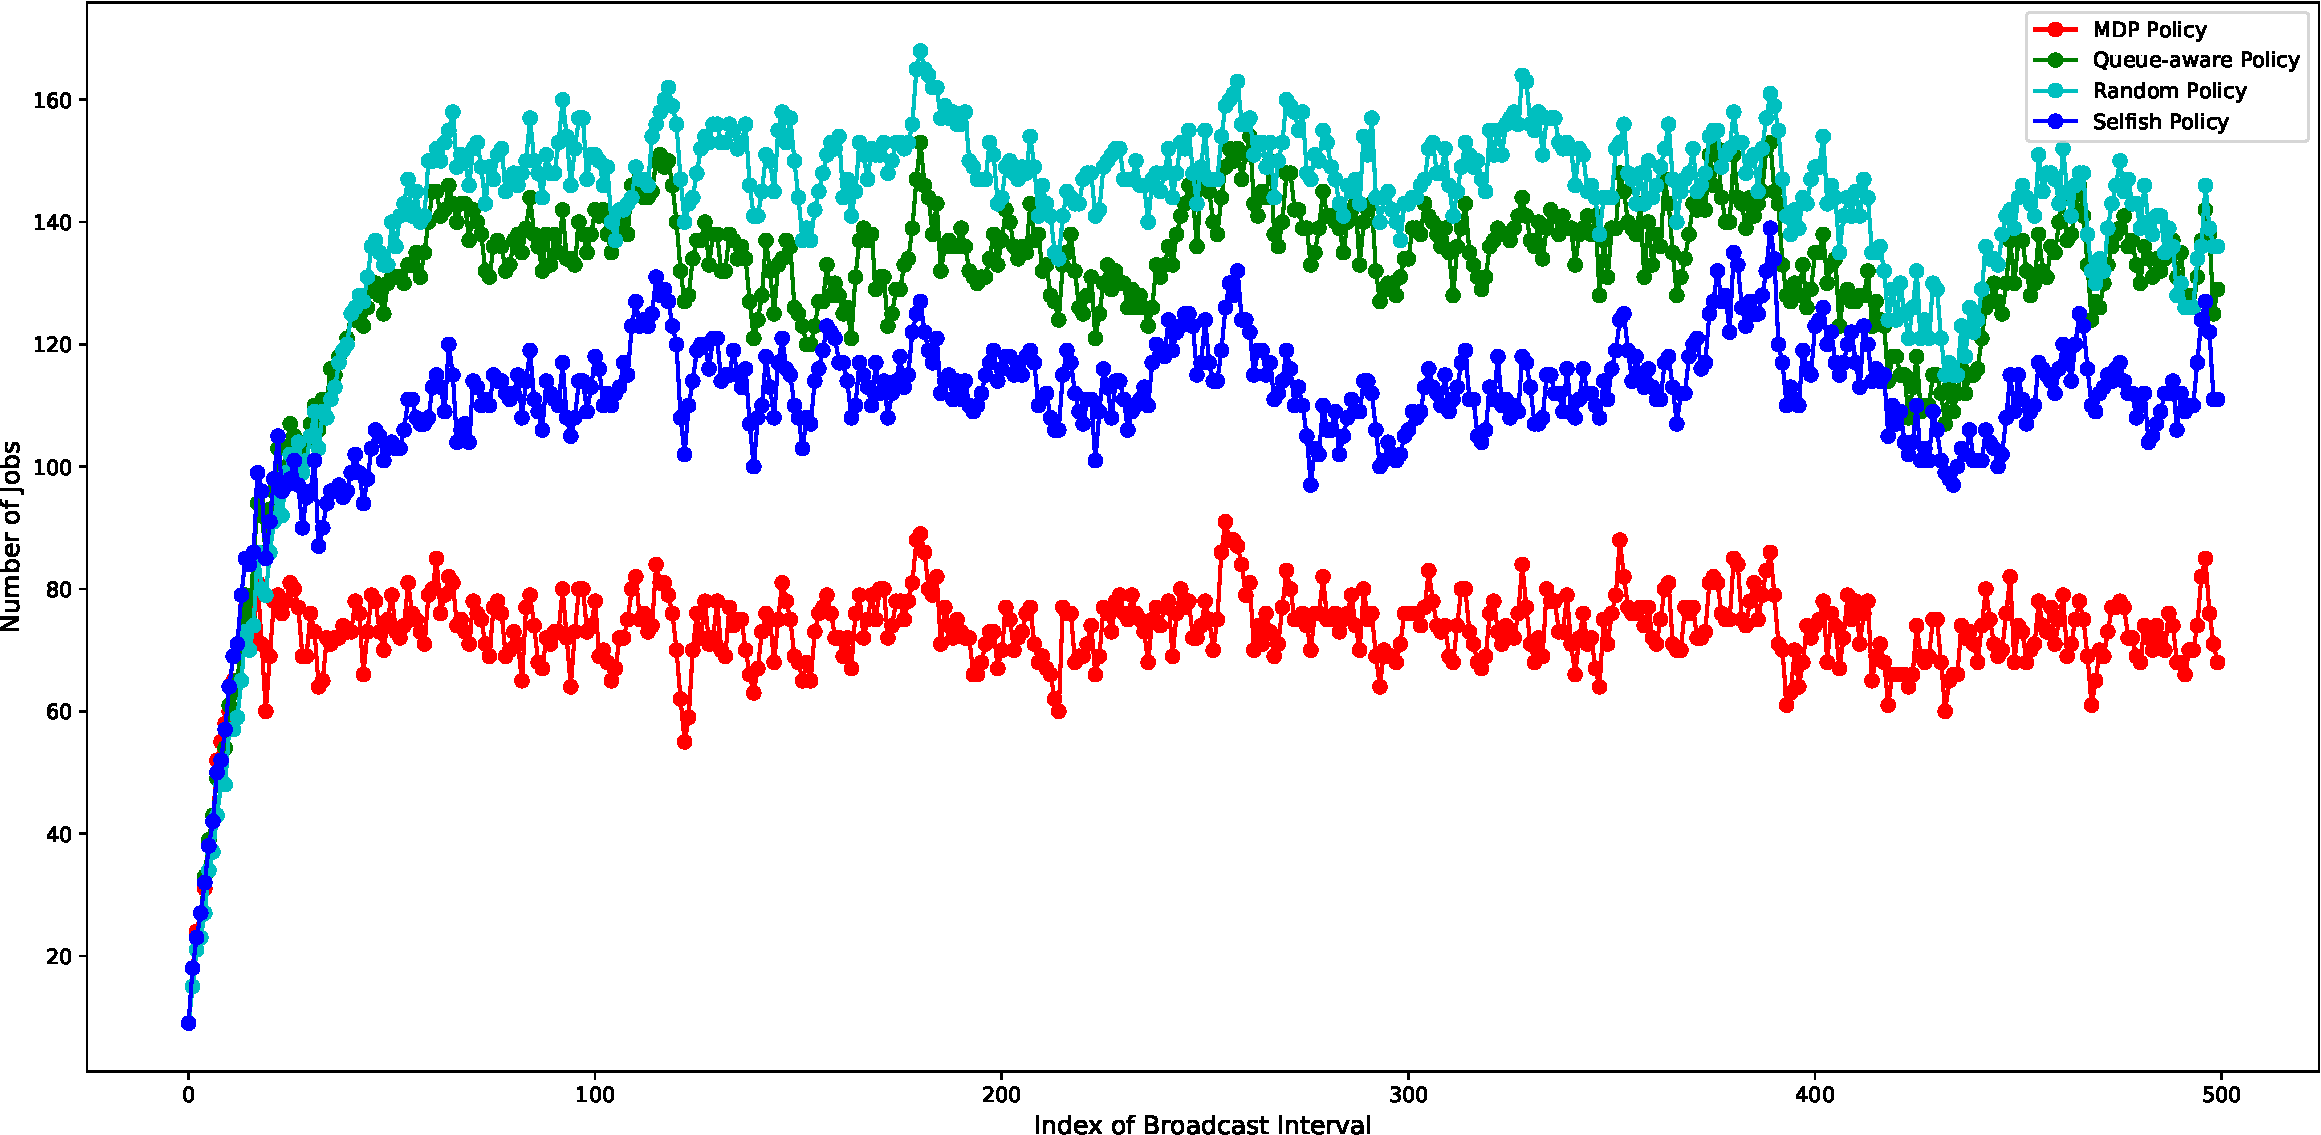
\includegraphics[width=0.80\textwidth]{41122-timeline-number.pdf}                           %
    \caption{Illustration of number of jobs on all the APs and edge servers over time.}         %
    \label{fig:general_timeline}                                                                %
\end{figure*}                                                                                   %
%-----------------------------------------------------------------------------------------------%

%NOTE: Benchmark Elaboration
\textbf{Benchmarks:}
We compare the proposed algorithm with other three heuristic algorithms which are listed as follows.
\begin{itemize}
    \item \textbf{Random Dispatching Policy}:
            for each job type, randomly choose the dispatching edge server in each time slot; 
    \item \textbf{Selfish Algorithm}:
            for each job type, always choose the edge server with the minimum expected uploading time, plus the expected processing time;
    \item \textbf{Queue-aware Selfish Algorithm}:
            for each job type, always choose the edge server with the minimum expected uploading time, plus the expected processing time and queueing time based on the observation of outdated queue states.
\end{itemize}
Specifically, we choose the \emph{Selfish Algorithm} which is state-invariant as the initial policy for our proposed algorithm.
The explicit definition is given as follows.
\begin{policy}[Selfish Policy]
    \begin{align}
        \Baseline &\define \Brace{ \Pi_{k}\define\set{\pi_{k,j}|\forall j\in\jSpace} |\forall k\in\apSet },
    \end{align}
    where $\pi_{k,j} \define \arg\min_{m\in\esSet_{k}} u_{k,m,j} + c_{m,j}$.
\end{policy}

%NOTE: Basic Performance
\subsection{Performance Analysis}
\label{subsec:basic}
The evaluation results are shown in Fig.\ref{fig:bar_plot} where three metrics are taken to demonstrate the performance of our proposed algorithm with other benchmarks.
\fixit{
    Average Cost v.s. Algorithms in Fig.\ref{fig:bar_plot}(a);
    Average JCT (job completion time) v.s. Algorithms, Fig.\ref{fig:bar_plot}(b);
    Average Departure Rate (throughput) v.s. Algorithms, Fig.\ref{fig:bar_plot}(c).
}
Specifically, our proposed algorithm is better than compared algorithms all the time in the timeline figure Fig.\ref{fig:brd-timeline}.
The CDF of cost is illustrated in Fig.\ref{fig:cdf_cost} where the cost of \emph{SQF policy} is nearly the same as the \emph{selfish policy}, however, the \emph{SQF policy} actually have very poor job departure rate (i.e. throughput) compared with the other's.
\fixit{
    This is because the broadcast information is periodically and outdated, and SQF could not handle the penalty brought by job rejection properly.
    And we take \emph{CDF of number of jobs} other than \emph{CDF of cost} which could better reflect the performance of the average JCT target in the simulation when job rejection considered.
    
}

%-----------------------------------------------------------------------%
\begin{figure}[ht]                                                      %
    \centering                                                          %
    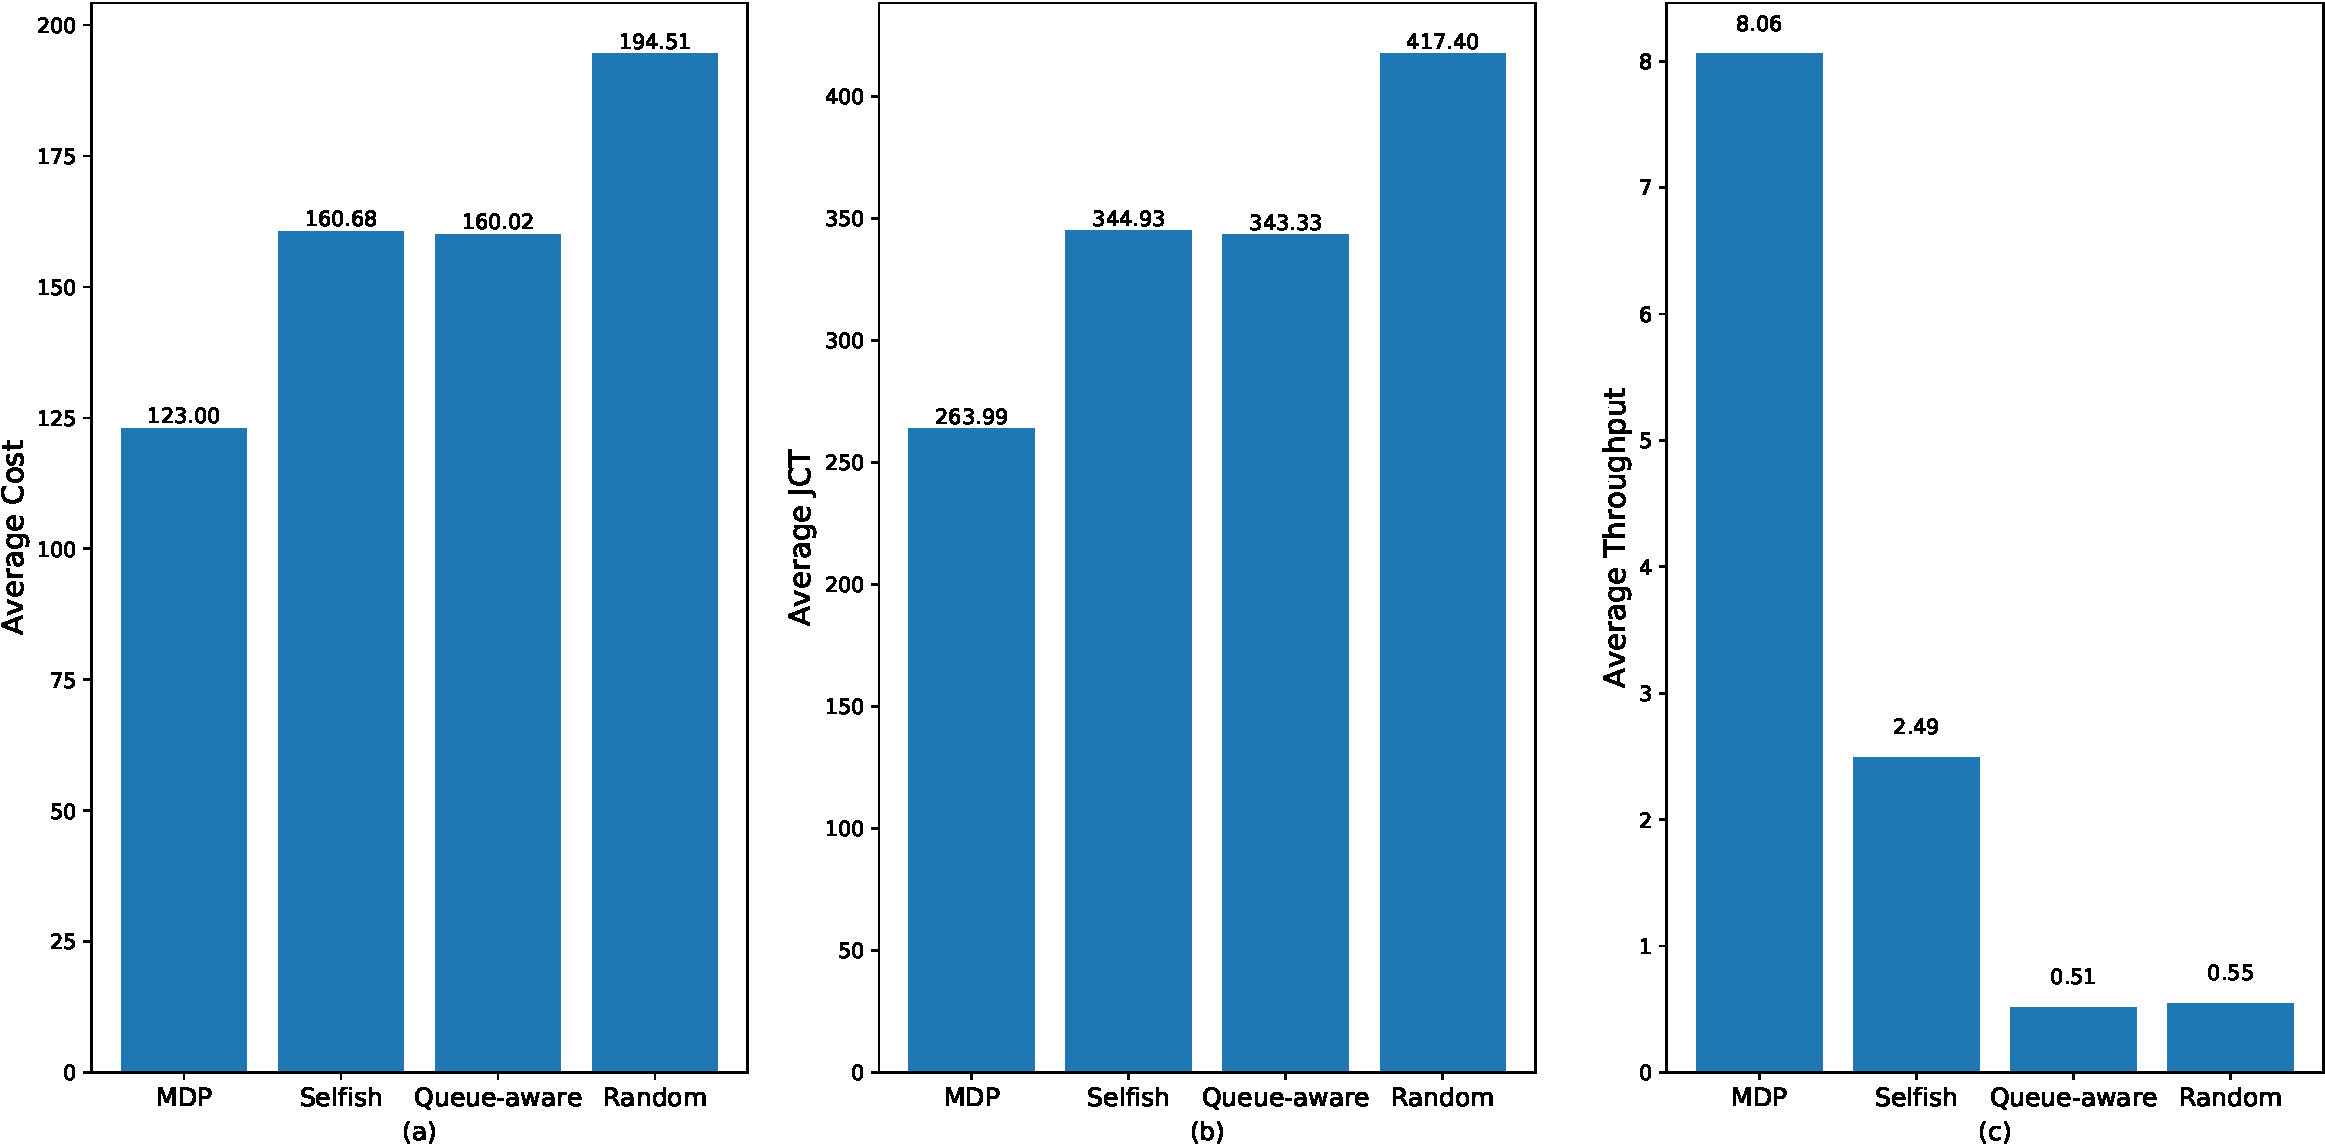
\includegraphics[width=0.45\textwidth]{41122-bar-graph.pdf}         %
    \caption{Illustration of performance metrics comparison with benchmarks.}
    \label{fig:bar_plot}                                                %
\end{figure}                                                            %
%-----------------------------------------------------------------------%
\begin{figure}[ht]                                                      %
    \centering                                                          %
    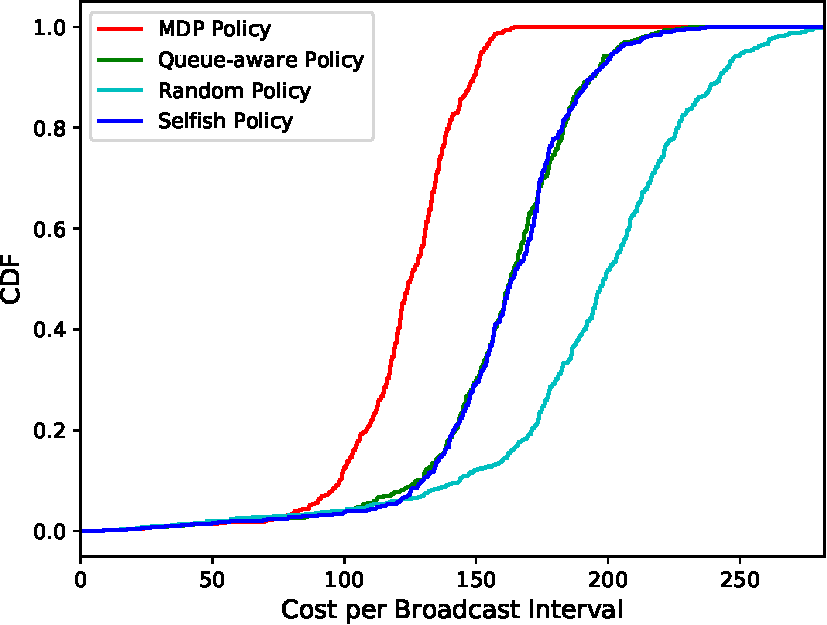
\includegraphics[width=0.45\textwidth]{41122-cdf-cost.pdf}          %
    \caption{Illustration of performance metrics comparison with benchmarks.}
    \label{fig:cdf_cost}                                                %
\end{figure}                                                            %
%-----------------------------------------------------------------------%
%----------------------------------------------------------------------------------------%
\subsection{Sensitivity Study}
\label{subsec:advance}  

%FIXME: replace the graphs
%-----------------------------------------------------------------------------------------------%
\begin{figure*}[ht!]                                                                            %
    \centering                                                                                  %
    \begin{tabular}{ccc}                                                                        %
        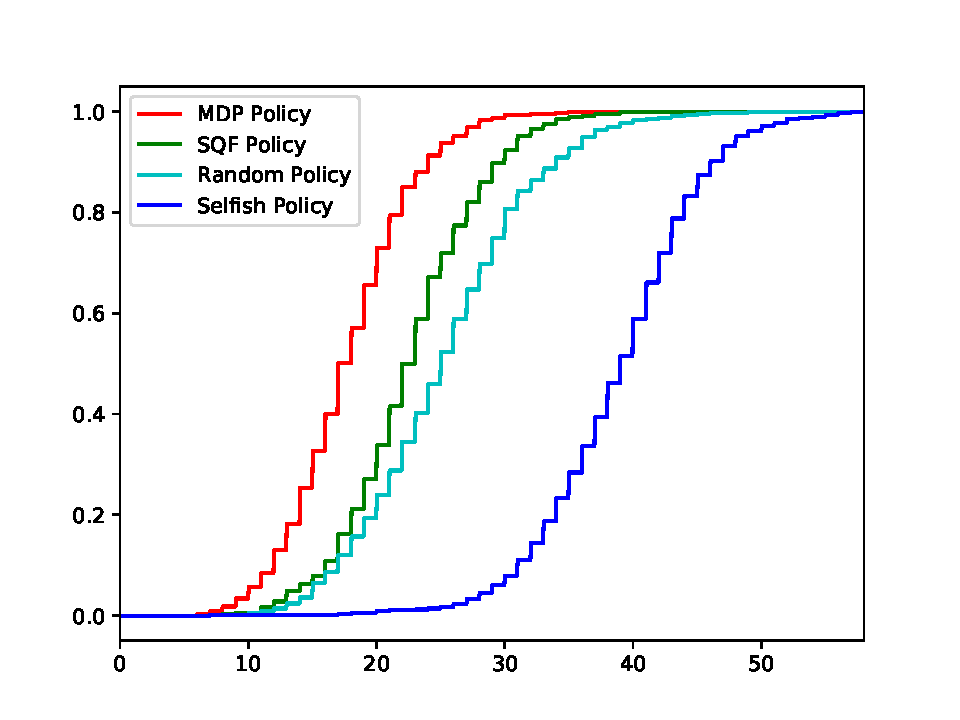
\includegraphics[width=0.30\textwidth]{images/535_LowPressure_NoDelay.pdf}&             %
        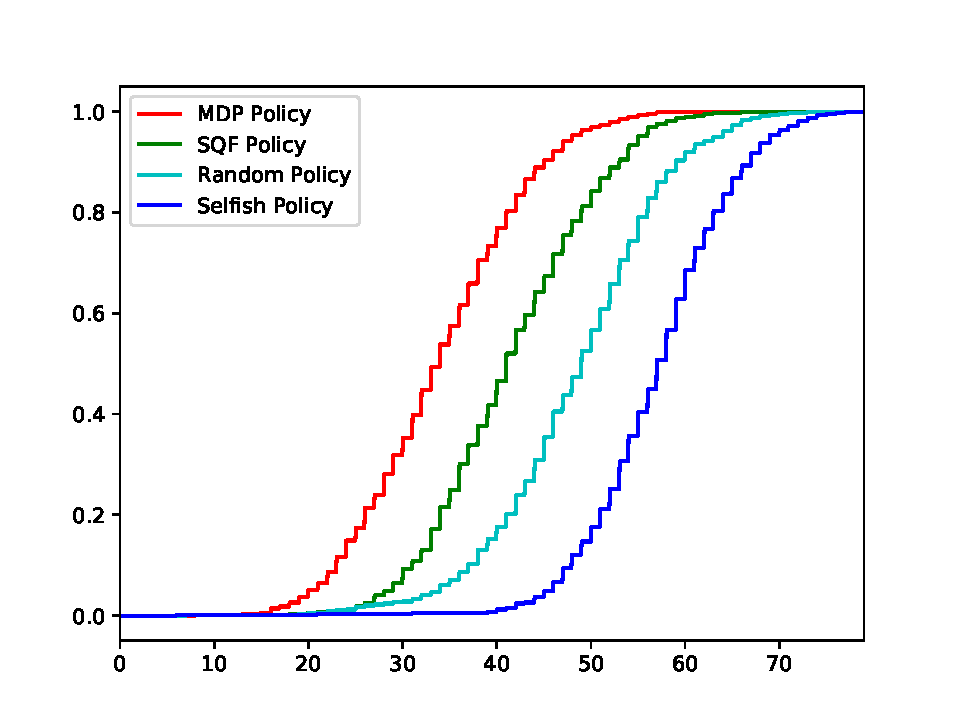
\includegraphics[width=0.30\textwidth]{images/535_LowPressure_LargeDelay_cdf.pdf}&      %
        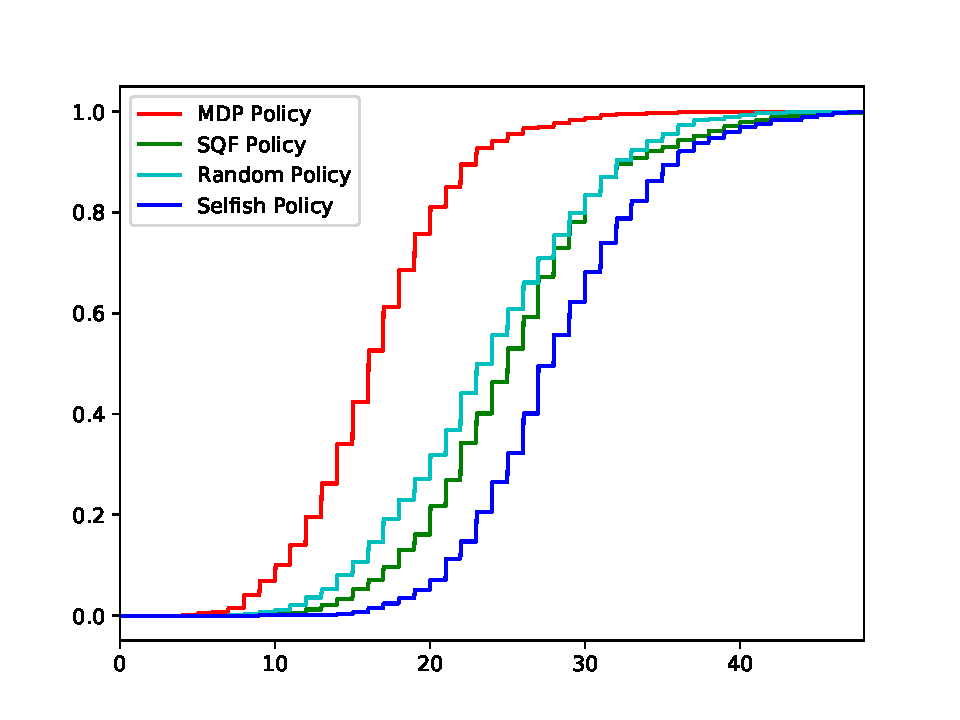
\includegraphics[width=0.30\textwidth]{images/535_LowPressure_FullDelay.pdf}            %
        \\                                                                                      %
        {\small (a) No \brlatency} &                                                            %
        {\small (b) Large \brlatency} &                                                         %
        {\small (c) Whole-interval \brlatency}                                                  %
    \end{tabular}                                                                               %
    \caption{Evaluation of Information Staleness Impact on Algorithm Robustness.}               %
    \label{fig:ss_delay}                                                                        %
\end{figure*}                                                                                   %
%-----------------------------------------------------------------------------------------------%

%-------------------------------------------------------------------%
\begin{figure}[hbt]                                                 %
    \centering                                                      %
    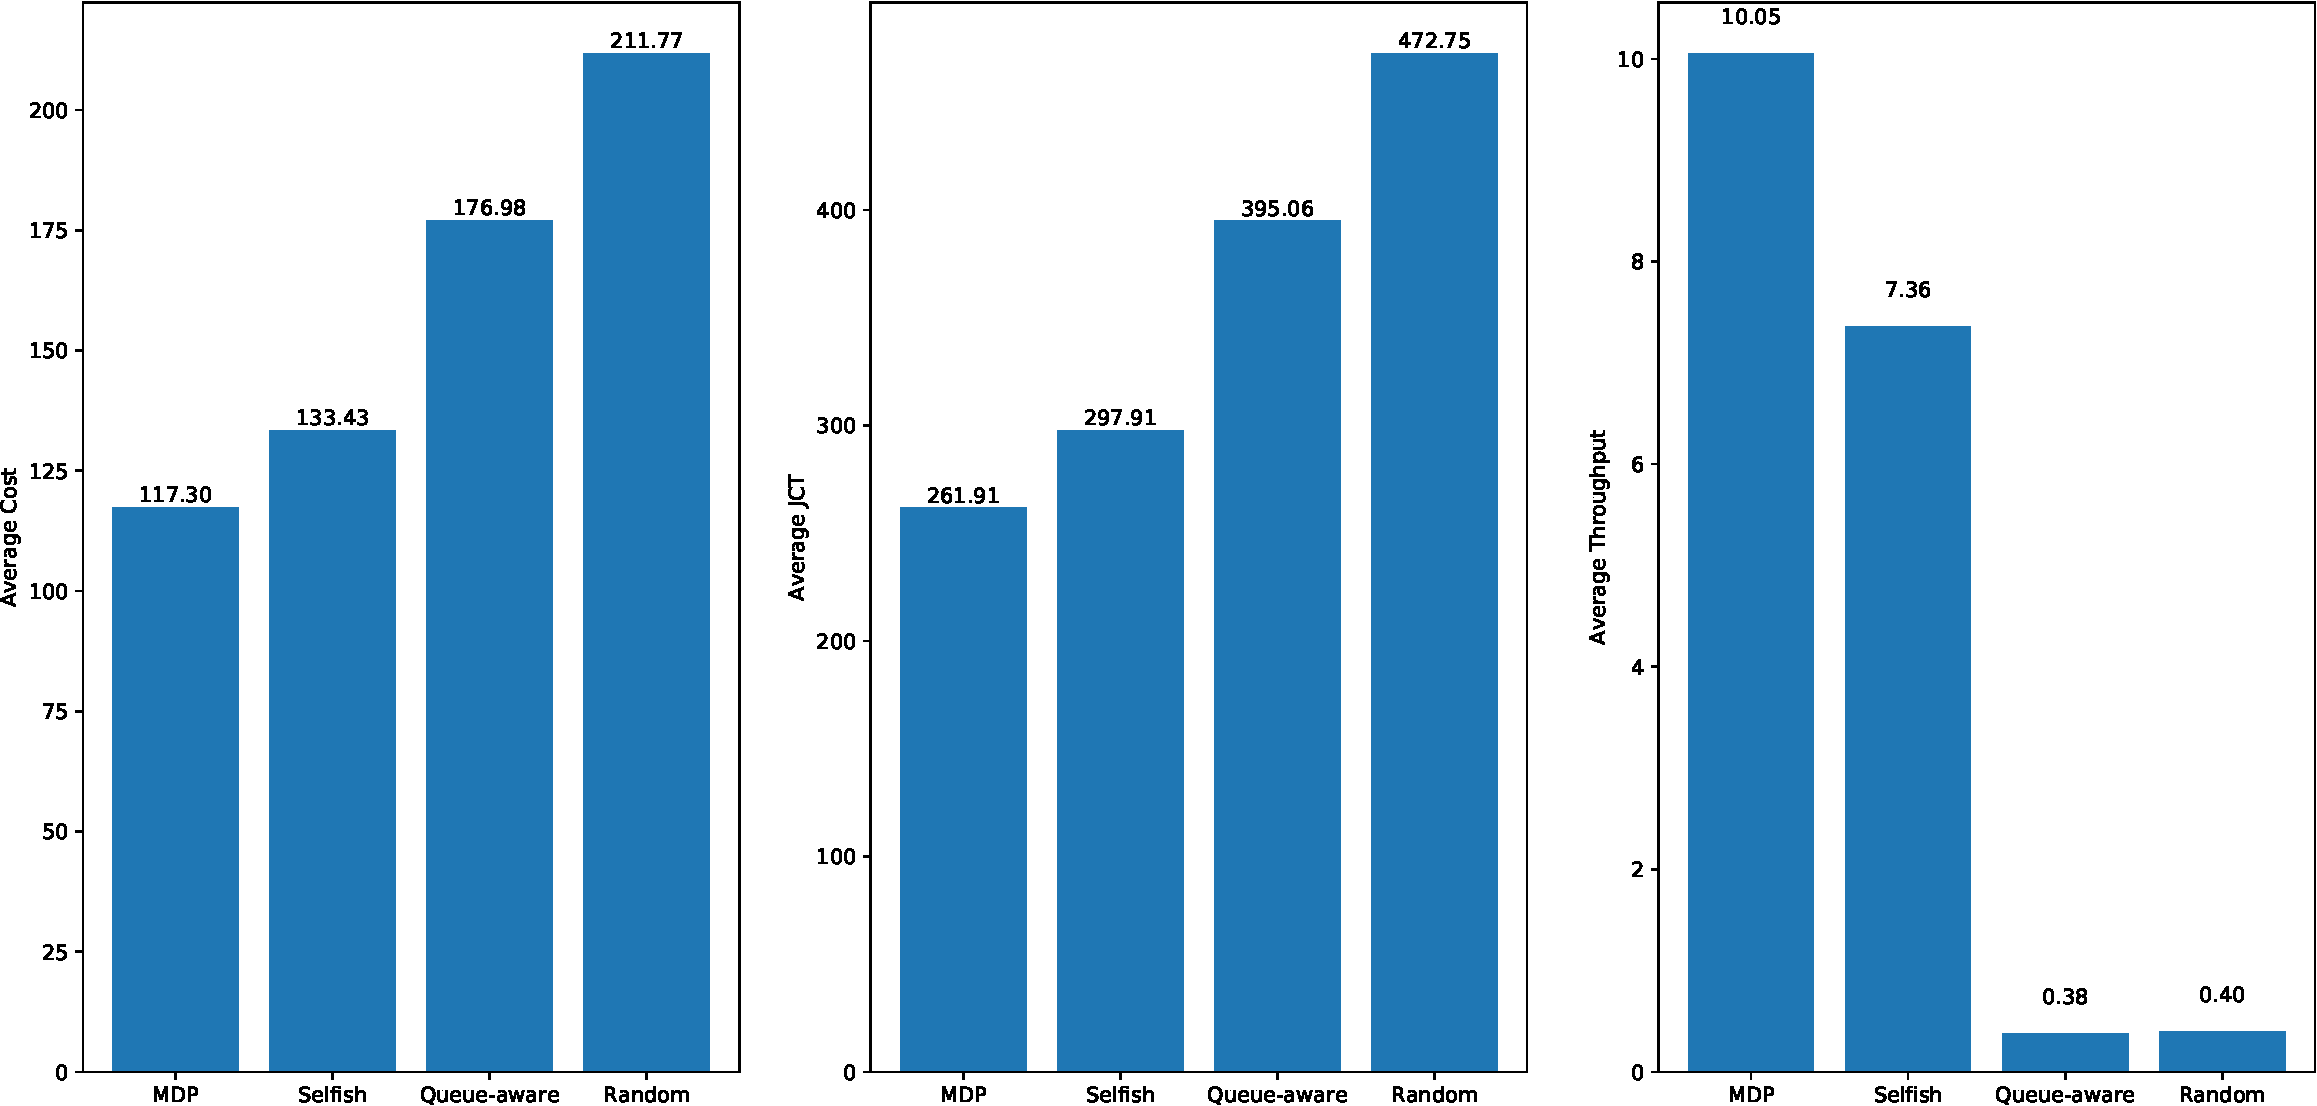
\includegraphics[width=0.45\textwidth]{bar_graph.pdf}           %
    \caption{Illustration of impact of scale of APs on algorithms.}
    \label{fig:ss_scale}                                            %
\end{figure}                                                        %
%-------------------------------------------------------------------%

%-------------------------------------------------------------------%
\begin{figure}[hbt]                                                 %
    \centering                                                      %
    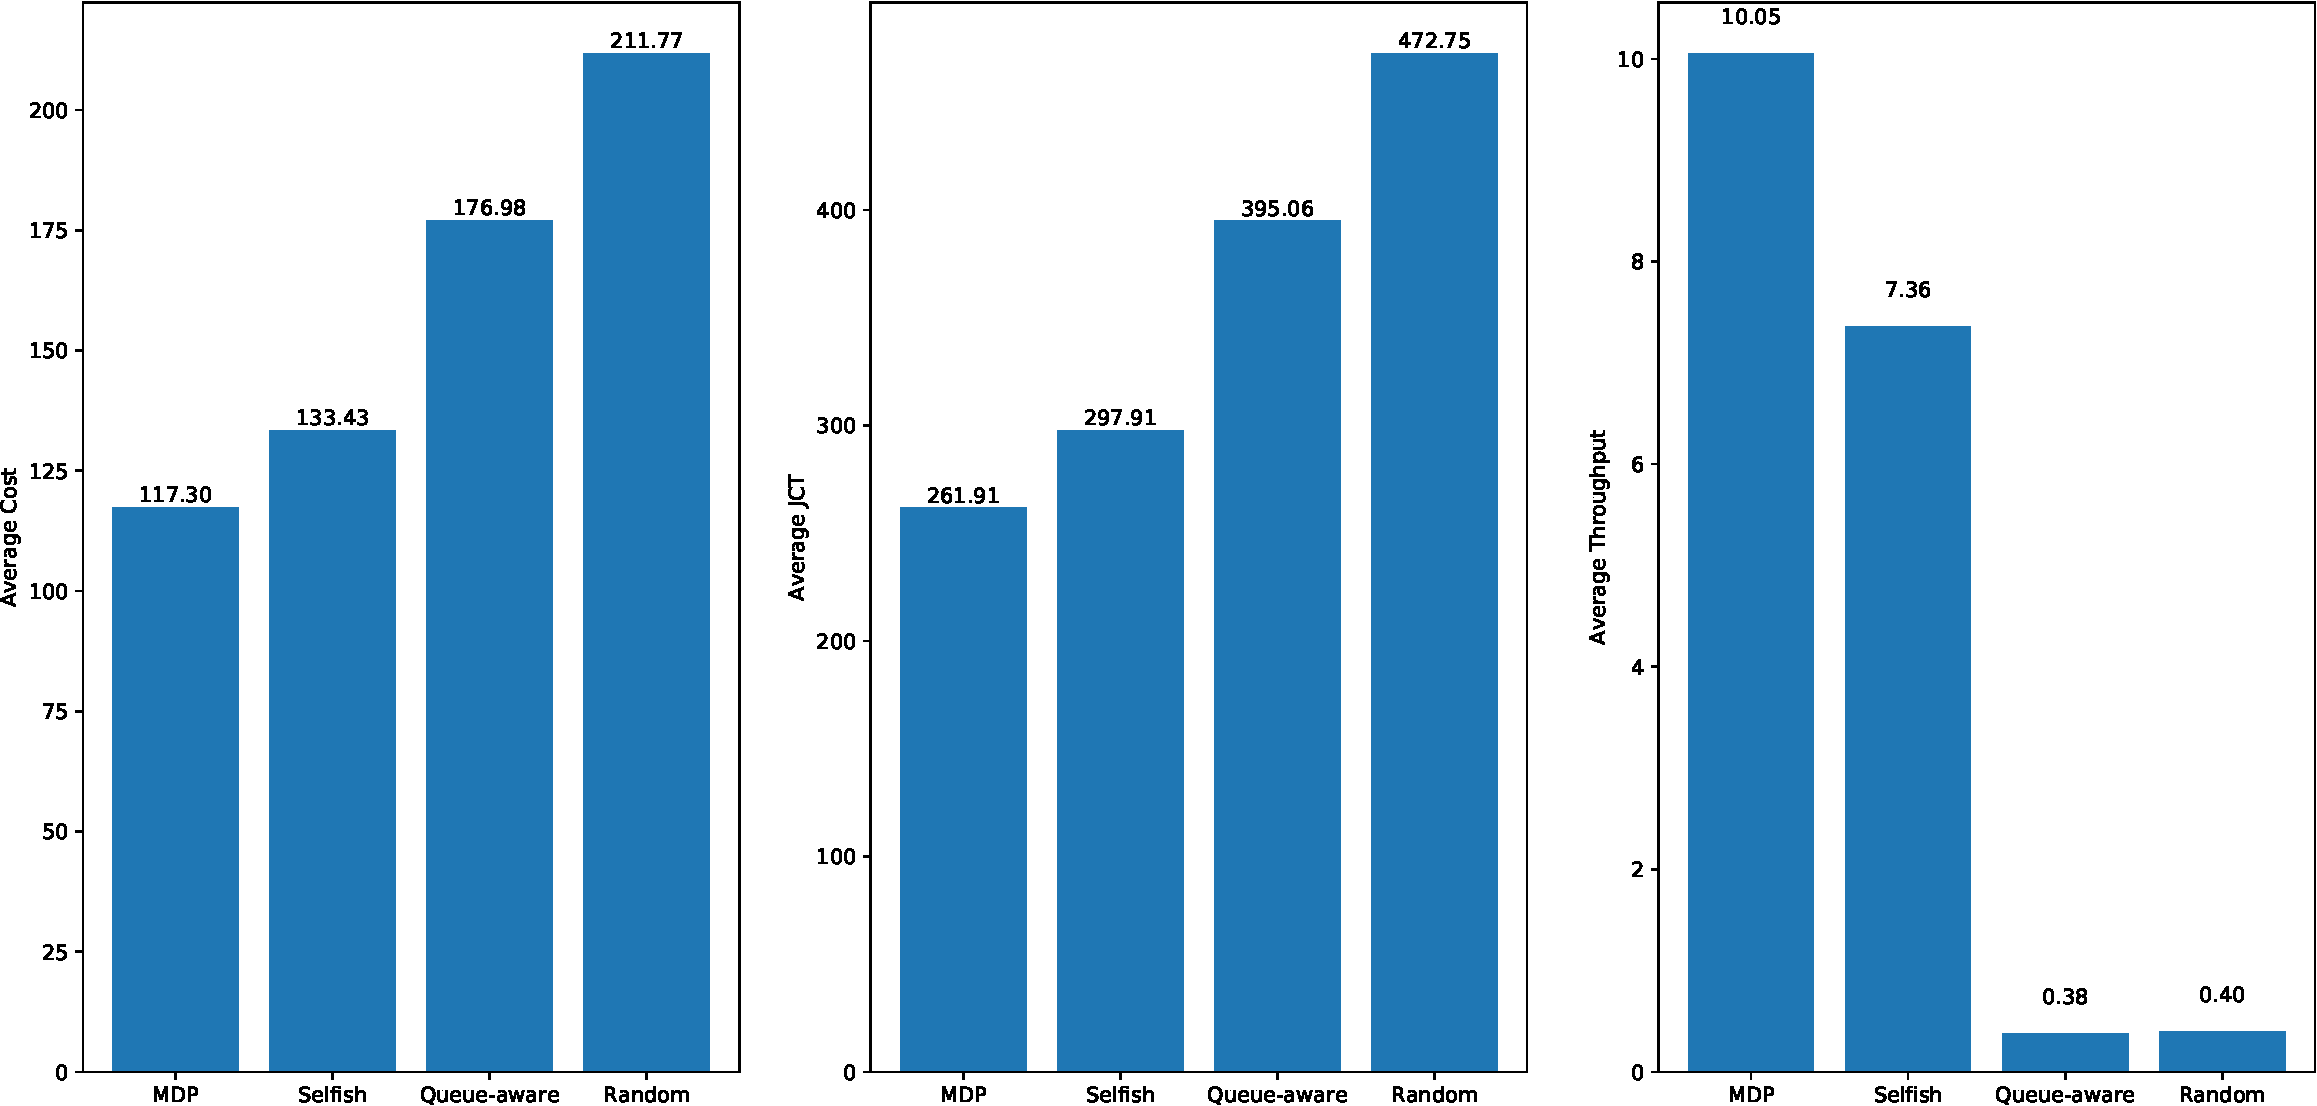
\includegraphics[width=0.45\textwidth]{bar_graph.pdf}           %
    \caption{Illustration of impact of uploading and processing time distribution on algorithms.}
    \label{fig:ss_dist}                                             %
\end{figure}                                                        %
%-------------------------------------------------------------------%

%-------------------------------------------------------------------%
\begin{figure}[hbt]                                                 %
    \centering                                                      %
    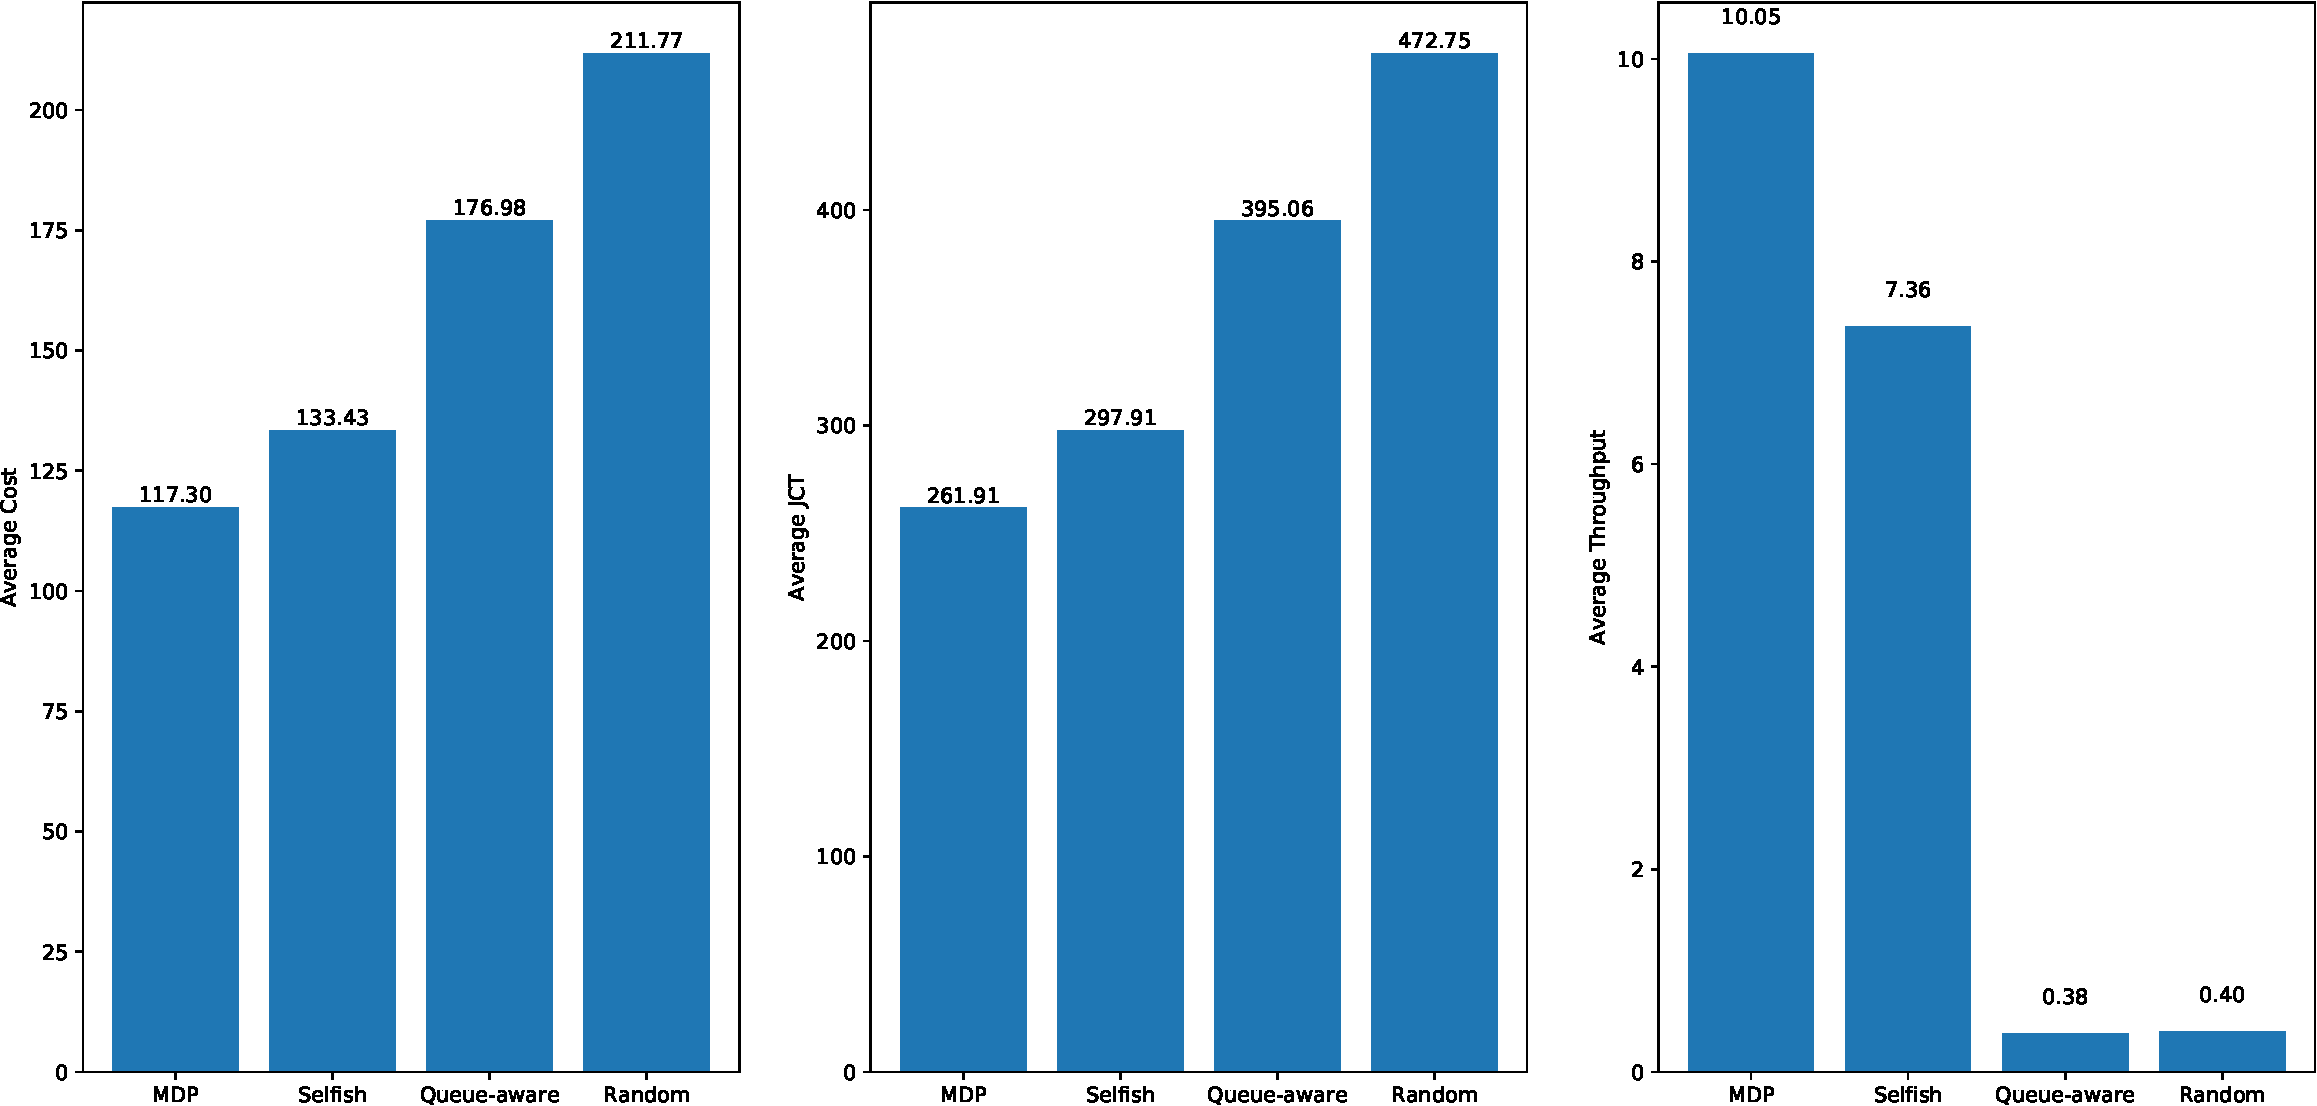
\includegraphics[width=0.45\textwidth]{bar_graph.pdf}           %
    \caption{Illustration of impact of penalty factors on algorithms.}
    \label{fig:ss_penalty}                                          %
\end{figure}                                                        %
%-------------------------------------------------------------------%

%NOTE: sensitivity study
\textbf{Various Signaling Latency.}
\fixit{
    The evaluation of staleness of \brlatency~is demonstrated in Fig.\ref{fig:ss_delay}.
}

\textbf{Number of APs.} %(a.k.a arrival rate)
The evaluation of scale of is demonstrated in Fig.\ref{fig:ss_scale}.
\fixit{
    It's shown that on the left of the figure, the SQF algorithm would work better when the system is almost idle; on the right of the figure, SQF and random algorithm could not handle high rejection rate and thus the \emph{average throughput} decreases extremely. 
}

\textbf{Uploading Time and Processing Time Distributions.}
\fixit{
    The evaluation of distribution of is demonstrated in Fig.\ref{fig:ss_dist}.
}

\textbf{Penalty Factors.}
\fixit{
    The evaluation of CDF of number of dropped jobs (over the queue limit) is shown in Fig.\ref{fig:ss_penalty}.
    % CDF of queue length.
}

%----------------------------------------------------------------------------------------%
